%%%% P218 Econometrics - Problem Set 1 %%%
%%%% Author: Will Hotten
\documentclass{article}

%%% Preamble
\usepackage[left=3cm,right=3cm]{geometry}
\usepackage{amsmath}
\usepackage{amssymb}
\usepackage{pgfplots}
\usepackage{hyperref}
\pgfplotsset{compat=1.16}

\hypersetup{
    colorlinks=true,
    linkcolor=blue,
    filecolor=magenta,      
    urlcolor=cyan,
    }

\setlength{\parindent}{0mm}

%%% Start of document
\begin{document}

%%%Title
\title{P218 Problem Set 1}
\author{Will Hotten}
\date{}
\maketitle

%%% Question 1 %%%
\section*{Question 1}

%% 1 - a %%
\subsection*{1.a.}
\begin{align*}
    \frac{\partial Y}{\partial X} 
    &= -2X + 2 + \varepsilon\\
    &=\left\{ \begin{array}{cl} -2X + 3 & \textrm{if }\varepsilon= 1\\
    -2X + 1 & \textrm{if }\varepsilon=-1 \end {array}\right.
\end{align*}

The causal effect of a marginal change in X on Y is always greater for farms with very good soil compared to those with very bad soil.

%% 1 - b %%
\subsection*{1.b.}
\begin{align*}
    ACE(X, \varepsilon)
    &= E[C(X, \varepsilon)|X]\\
    &= \int_{-1}^{1} \frac{\partial}{\partial X}Y(X,\varepsilon)
    \cdot f_{\varepsilon \mid X}(\varepsilon \mid X) \,d\varepsilon
    \\
\end{align*}

For this we need to calculate the density of X conditional on $\varepsilon$:
\begin{align*}
    f_{\varepsilon \mid X}(\varepsilon \mid X)
    &= \frac{f_{X\varepsilon}(x,\varepsilon)}{f_{X}(x)}\\
    &= \left(\frac{1+x-\varepsilon}{8}\right)\cdot\left(\frac{1}{f_{X}(x)}\right)
    \\
\end{align*}

To calculate the marginal density of X:
\begin{align*}
    f_{X}(x)
    &=\int_{-1}^{1}\left(\frac{1+x-\varepsilon}{8}\right) \,d\varepsilon \\
    &=\left[\frac{-\varepsilon(1+x)}{8}+\frac{-\varepsilon^2}{16}\right]_{-1}^{1}\\
    &=-\left[\frac{1+x}{8} + \frac{1}{16}\right]
    + \left[-\frac{1+x}{8} + \frac{1}{16}\right]\\
    &= \frac{1+x}{4}
\end{align*}

Therefore, the conditional density can be rewritten:
\begin{align*}
    f_{\varepsilon \mid X}(\varepsilon \mid X)
    &= \left(\frac{1+x-\varepsilon}{8}\right)\cdot\left(\frac{4}{1+x}\right)\\
    &= \frac{1}{2} \cdot \left(\frac{1+x-\varepsilon}{1+x}\right)\\
\end{align*}

Plugging this into the formula for ACE(X,$\varepsilon$):
\begin{align*}
    ACE(X, \varepsilon)
    &= \int_{-1}^{1} \frac{\partial}{\partial X}Y(X,\varepsilon)\cdot \frac{1}{2} \cdot \left(\frac{1+x-\varepsilon}{1+x}\right) \,d\varepsilon \\
    &= \int_{-1}^{1} \frac{1}{2}\cdot (-2x + 2 + \varepsilon)\cdot 
    \left(\frac{1+x-\varepsilon}{1+x}\right) \,d\varepsilon \\
    &= \left[\frac{-\varepsilon\cdot\left(\varepsilon\cdot\left(2\varepsilon-9x+3\right)+12x^2-12\right)}{12\left(x+1\right)}\right]_{-1}^{1} \\
    &= \left[\frac{-12x^2 + 9x + 13}{12(x+1)}\right]
    - \left[\frac{12x^2 + 9x + 7}{12(x+1)}\right] \\
    &= \frac{5-6x^2}{3x+3}
\end{align*}

Plotting ACE(X,$\varepsilon$):

\begin{figure}[!h]
\centering
\begin{tikzpicture}
\centering
    \begin{axis}[
        xlabel=$x$,
        xmin=0, xmax=2,
        ymin=-3, ymax=3,
        xtick={0,1,2},   
        ytick={-3, -19/9, 0, 5/3, 3}
                ]
      
    \addplot+[mark=none] {(5-6*(x^2))/((3*x)+3)};
    
    \addlegendentry{ACE}
    \end{axis}
\end{tikzpicture}
\end{figure}

The average causal effect of X on Y is decreasing in X.

%% 1 - c %%
\subsection*{1.c.}
E(Y):
\begin{align*}
    E(Y)
    &= E(-X^2 + 2X + \varepsilon X)\\
    &= -E(X^2) + 2E(X) + E(\varepsilon X)\\
\end{align*}

Now, $E(X$):
\begin{align*}
    E(X)
    &= \int_{0}^{2}xf_{x}(x) \,dx \\
    &= \int_{0}^{2}x \frac{1+x}{4}\\
    &= \frac{1}{4} \left[\frac{x^2}{2} + \frac{x^3}{3} \right]_{0}^{2}\\
    &= \frac{7}{6}\\
\end{align*}

$E(X^2)$:
\begin{align*}
    E(X^2)
    &= \int_{0}^{2}x^2 f_{x}(x) \,dx \\
    &= \int_{0}^{4}x^2 \frac{1+x}{4}\\
    &= \frac{1}{4} \left[\frac{x^3}{3} + \frac{x^4}{4} \right]_{0}^{4}\\
    &= \frac{5}{3}\\
\end{align*}

$E(\varepsilon X)$:
\begin{align*}
    E(\varepsilon X)
    &= \int_{-1}^{1}\int_{0}^{2}x\varepsilon f_{x \varepsilon}(x, \varepsilon) \,dx \,d\varepsilon\\
    &= \int_{-1}^{1} \left[\frac{\varepsilon x^2\cdot\left(2x-3\varepsilon+3\right)}{48} \right]_{0}^{2} \,d\varepsilon\\
    &= \int_{-1}^{1} -\frac{\varepsilon \cdot\left(6\varepsilon -14\right)}{24} \,d\varepsilon\\
    &= \left[-\frac{\varepsilon ^2\cdot\left(2 \varepsilon -7\right)}{24} \right]_{-1}^{1}\\
    &= -\frac{1}{6}\\
\end{align*}

Putting together:
\begin{align*}
    E(Y)
    &= -\frac{5}{3} + 2\left(\frac{7}{6}\right) + -\frac{1}{6}\\
    &= \frac{1}{6} \cdot \left(-10 + 14 - 1\right) \\
    &= \frac{1}{2}\\
\end{align*}

E(Y $\mid$ X):
\begin{align*}
    E(Y \mid X)
    &= E(-X^2 + 2X + \varepsilon X \mid X)\\
    &= -X^2 + 2X + XE(\varepsilon \mid X)\\
\end{align*}

From earlier:
\begin{align*}
    f_{\varepsilon \mid X}(\varepsilon \mid X)
    &= \frac{1}{2} \cdot \left(\frac{1+x-\varepsilon}{1+x}\right)\\
\end{align*}

Therefore, $E(\varepsilon \mid X)$:
\begin{align*}
    E(\varepsilon \mid X)
    &= \int_{-1}^{1}\varepsilon f_{\varepsilon \mid X}(\varepsilon \mid X) \,d\varepsilon \\
    &= \int_{-1}^{1}\varepsilon \frac{1+x-\varepsilon}{2(1+x)} \,d\varepsilon \\
    &= \left[ -\frac{\varepsilon^2\cdot\left(2\varepsilon-3x-3\right)}{12\left(x+1\right)}\right]_{0}^{2}\\
    &= -\frac{1}{3x+3}\\
\end{align*}

E(Y $\mid$ X):
\begin{align*}
    E(Y \mid X)
    &= -X^2 + 2X + XE(\varepsilon \mid X)\\
    &= -X^2 + 2X - \left(\frac{X}{3X+3}\right)\\
\end{align*}

%% 1 - d %%
\subsection*{1.d.}
\begin{align*}
    \frac{\partial}{\partial X}E(Y \mid X)
    &= \frac{\partial}{\partial X}\left(-X^2 + 2X - \left(\frac{X}{3X+3}\right)\right)\\
    &= -2X + 2 - \frac{1}{3(X+1)^2}\\
\end{align*}

Compared to ACE(X,$\varepsilon$):
\begin{align*}
    ACE(X, \varepsilon)
    &= \frac{5-6x^2}{3x+3}
\end{align*}

\begin{figure}[!h]
\centering
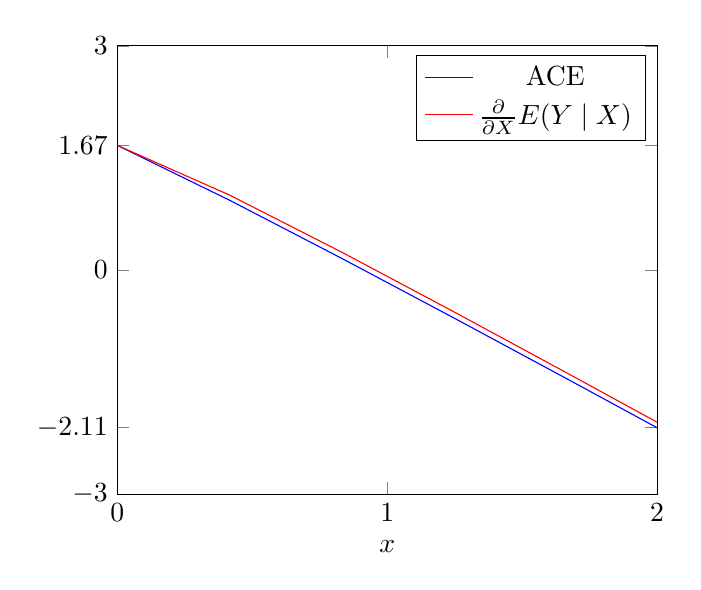
\begin{tikzpicture}
\centering
    \begin{axis}[
        xlabel=$x$,
        xmin=0, xmax=2,
        ymin=-3, ymax=3,
        xtick={0,1,2},   
        ytick={-3, -19/9, 0, 5/3, 3}
                ]
      
    \addplot+[mark=none] {(5-6*(x^2))/((3*x)+3)};
    \addplot+[mark=none] {-2*x + 2 - (1/(3*(x+1)^2))};
    
    \addlegendentry{ACE}
    \addlegendentry{$\frac{\partial}{\partial X}E(Y \mid X)$}
    \end{axis}
\end{tikzpicture}
\end{figure}

As we can see from the plot there is only a small difference between $\frac{\partial}{\partial X}E(Y \mid X)$ and ACE(X,$\varepsilon$).

Here it appears that $\frac{\partial}{\partial X}E(Y \mid X)$ and ACE(X,$\varepsilon$) are very similar over the set of possible X values. This would suggest that our regression estimates may be interpreted as estimates of the causal impact of X on Y.

%% 1 - e %%
\subsection*{1.e.}
The BLP of Y given X solves:

\begin{align*}
    \min\limits_{\alpha , \beta} E(Y - \alpha - \beta X)^2
\end{align*}

Solution:
\begin{align*}
    \beta^{*} &= \frac{Cov(X, Y)}{Var(X)} \\
    \alpha^{*} &= E(Y) - \beta^{*} E(X) 
\end{align*}

$E(X)$, $E(X^2)$, $E(Y \mid X)$ and $E(Y)$:
\begin{align*}
    E(X) &= \frac{7}{6} \\
    E(X^2) &= \frac{5}{3} \\
    E(Y \mid X) &= -X^2 + 2X - \left(\frac{X}{3X+3}\right)\\
    E(Y) &= \frac{1}{2}
\end{align*}

Cov(X, Y):
\begin{align*}
    Cov(X, Y)
    &= E(XY) - E(X)E(Y)\\
    &= E[X E(Y \mid X)] - E(X)E(Y)\\
    &= E\left[-X^3 + 2X^2 - \left( \frac{X^2}{3X + 3} \right) \right] - \frac{7}{12} \\
    &= \int_{0}^{2}\left(-X^3 + 2X^2 -  \frac{X^2}{3X + 3} \right) \cdot \left( \frac{1+x}{4} \right) \,dx - \frac{7}{12}\\
    &= \frac{23}{45} - \frac{7}{12} \\
    &= -\frac{13}{180}
\end{align*}

Var(X, Y):
\begin{align*}
    Var(X)
    &= E(X^2) - E(X)^2\\
    &= \frac{5}{3} - \frac{49}{36} \\
    &= \frac{11}{36}
\end{align*}

So the BLP estimates are:
\begin{align*}
    \beta^{*} &= \frac{Cov(X, Y)}{Var(X)} 
    = \frac{-\frac{13}{180}}{\frac{11}{36}}
    = -\frac{13}{55} \\
    \alpha^{*} &= E(Y) - \beta^{*} E(X) 
    = \frac{1}{2} + \frac{13}{55} \cdot \frac{7}{6}
    = \frac{128}{165}
\end{align*}

OLS of Y on constant and X estimates the BLP as the OLS estimates are the sample analogs of the first order conditions that characterise the solution to the BLP.

%%% Question 2 %%%
\clearpage
\section*{Question 2}

%% 2 - a %%
% Showing that Beta tilde is linear
\subsection*{2.a}
\begin{align*}
    \Tilde{\beta}
    &= \frac{\bar{Y}}{\bar{X}}\\
    &= \frac{\frac{1}{n}\sum_{i=1}^{n} Y_{i}}{\frac{1}{n}\sum_{i=1}^{n} X_{i}}\\
    &= \left(\frac{1}{\sum_{i=1}^{n} X_{i}}\right) \cdot \sum_{i=1}^{n} Y_{i}\\
    &= g\left(\sum_{i=1}^{n} Y_{i}\right)
\end{align*}

This is a linear function of Y, therefore $\Tilde{\beta}$ is a linear estimator.

% Showing that beta tilde is conditionally unbiased
\begin{align*}
    E(\Tilde{\beta} \mid X)
    &= E\left(\frac{\bar{Y}}{\bar{X}} \mid X\right)\\
    &= \frac{1}{n\bar{X}} E \left(n\bar{Y} \mid X \right)\\
    &= \frac{1}{n\bar{X}} E \left({\sum_{i=1}^{n} X_{i}\beta + \varepsilon} \mid X \right)\\
    &= \frac{1}{n\bar{X}} \left(E({\sum_{i=1}^{n} X_{i}\beta + \varepsilon}) \mid X \right)\\
    &= \frac{1}{n\bar{X}} \left({\sum_{i=1}^{n} X_{i}\beta + 0} \right)\\
    &= \frac{1}{n\bar{X}} \left(\beta{\sum_{i=1}^{n} X_{i}} \right)\\
    &= \beta\frac{n\bar{X}}{n\bar{X}} \\
    &= \beta
\end{align*}

$\Tilde{\beta}$ is conditionally unbiased.

% Calculating conditional variance
\begin{align*}
    Var(\Tilde{\beta} \mid X)
    &= Var\left(\frac{\bar{Y}}{\bar{X}} \mid X\right)\\
    &= \frac{1}{n^2\bar{X}^2} Var \left(n\bar{Y} \mid X \right)\\
    &= \frac{1}{n^2\bar{X}^2} Var \left({\sum_{i=1}^{n} Y_{i}} \mid X \right)\\
    &= \frac{1}{n^2\bar{X}^2} Var \left({\sum_{i=1}^{n} X_{i}\beta + \varepsilon} \mid X \right)\\
    &= \frac{1}{n^2\bar{X}^2} \left({\sum_{i=1}^{n} Var(X_{i}\beta + \varepsilon \mid X )} \right)\\
    &= \frac{1}{n^2\bar{X}^2} \left(\beta^2{\sum_{i=1}^{n} Var(X_{i} \mid X) + \sum_{i=1}^{n}Var(\varepsilon \mid X )} \right)\\
    &= \frac{1}{n^2\bar{X}^2} \left(0 + \sum_{i=1}^{n}\sigma^2 \right)\\
    &= \frac{\sigma^2}{\bar{X}\sum_{i=1}^{n}X_{i}^}\\
\end{align*}

% Compare to the conditional variance of OLS
Compare to the conditional variance of the OLS estimator:
\begin{align*}
    Var(\hat{\beta}^{OLS} \mid X)
    &= \sigma^2 (X'X)^{-1}\\
    &= \frac{\sigma^2}{\sum_{i=1}^{n}X_{i}^2}
\end{align*}

% Comparison
$Var(\hat{\beta}^{OLS} \mid X)$ is smaller than $Var(\Tilde{\beta} \mid X)$ as $\sum_{i=1}^{n}X_{i}^2$ is greater than $\bar{X} \sum_{i=1}^{n} X_{i}$.

%% 2 - b %%
% Using first m observations and doing OLS
\subsection*{2.b}
\begin{align*}
    \hat{\beta}_{(m)}
     &= \frac{\sum_{i=1}^{m} (x_{i} - \bar{x}) (y_{i} - \bar{y})}{\sum_{i=1}^{m} (x_{i} - \bar{x})^2} \\
     &= (X_{m}'X_{m})^{-1} (X_{m}'Y_{m})
\end{align*}

This estimator is linear in y.

\begin{align*}
    E[\hat{\beta}_{(m)} \mid X]
    &= E[(X_{m}'X_{m})^{-1} (X_{m}'Y_{m}) \mid X] \\
    &= (X_{m}'X_{m})^{-1} X_{m}'E[Y_{m} \mid X] \\
    &= (X_{m}'X_{m})^{-1} X_{m}'X_{m}\beta \\
    &= \beta
\end{align*}

Thus, $\hat{\beta}_{(m)}$ is conditionally unbiased.
\begin{align*}
    Var(\hat{\beta}_{(m)} \mid X)
    &= Var((X_{m}'X_{m})^{-1} (X_{m}'Y_{m}) \mid X) \\
    &= (X_{m}'X_{m})^{-1} X_{m}' Var(Y_{m} \mid X) X_{m} (X_{m}'X_{m})^{-1} \\
    &= (X_{m}'X_{m})^{-1} X_{m}' \sigma^2 I_{m} X_{m} (X_{m}'X_{m})^{-1} \\
    &= \sigma^2 (X_{m}'X_{m})^{-1} X_{m}'X_{m} (X_{m}'X_{m})^{-1} \\
    &= \sigma^2 (X_{m}'X_{m})^{-1} \\
\end{align*}

The unconditional variance of the OLS estimator using all n observations is:
\begin{align*}
    Var(\hat{\beta} \mid X)
    &= \sigma^2 (X'X)^{-1} \\
\end{align*}

Comparing variances:
\begin{align*}
    (X_{m}'X_{m})^{-1} 
    &= \frac{1}{\sum_{i=1}^{m} x_{i}^2} \\
    (X'X)^{-1}
    &= \frac{1}{\sum_{i=1}^{n} x_{i}^2}
\end{align*}

$Var(\hat{\beta}_{(m)} \mid X)$ $\ge$ $Var(\hat{\beta} \mid X)$ as $\sum_{i=1}^{m}x_{i}^2$ $\le$ $\sum_{i=1}^{n}x_{i}^2$

%% 2 - c %%
% Suggesting a minimum conditional variance, linear estimator
\subsection*{2.c}

A minimum conditional variance, linear estimator could simply be a constant function such as $\hat{\beta} = 1$. This is both linear and has zero variance.


%%% Question 3 %%%
\clearpage
\section*{Question 3}

%% 3 - a %%
\subsection*{3.a}

Only one observation of (y,x) available, so the OLS estimate simplifies to:

% Defining OLS estimator
\begin{align*}
    \hat{\beta}^{OLS}
    &= (X'X)^{-1}X'Y\\
    &= \frac{xy}{x}\\
    &= \frac{y}{x}
\end{align*}

Calculating the unconditional mean of the estimator:
\begin{align*}
    E(\hat{\beta}^{OLS})
    &= E\left(\frac{y}{x}\right)\\
    &= E\left(\frac{\beta x + \varepsilon}{x}\right)\\
    &= E(\beta) + E\left(\frac{\varepsilon}{x}\right)\\
    &= \beta + E(\varepsilon) \cdot E\left(\frac{1}{x}\right)\\
    &= \beta
\end{align*}

Calculating the unconditional variance of the estimator:
\begin{align*}
    Var(\hat{\beta}^{OLS})
    &= Var\left(\frac{y}{x}\right)\\
    &= Var\left(\frac{\beta x + \varepsilon}{x}\right)\\
    &= Var\left(\beta + \frac{\varepsilon}{x}\right)\\
    &= E\left[\left(\beta + \frac{\varepsilon}{x}\right)^2\right] 
    - E\left[\beta + \frac{\varepsilon}{x}\right]^2\\
    &= E\left[\beta^2 + 2\beta \frac{\varepsilon}{x} + \frac{\varepsilon^2}{x^2} \right]
    - \beta^2\\
    &= \beta^2 + 2\beta E\left[\frac{1}{x}\right] E[\varepsilon] + E\left[\frac{1}{x^2}\right] E[\varepsilon^2] - \beta^2\\
    &= \beta^2 + \frac{625}{49} - \beta^2\\
    &= \frac{625}{49}
\end{align*}

\subsection*{3.b}

% Calculating unconditional bias of beta tilde
\begin{align*}
    E(\tilde{\beta})
    &= E\left(xy\right)\\
    &= E(\beta x^2 + \varepsilon x)\\
    &= \beta E(x^2) + E(\varepsilon x)\\
    &= \beta E(x^2) + E(\varepsilon)E(x)\\
    &= \beta(1) + 0\\
    &= \beta
\end{align*}

$\Tilde{\beta}$ is unconditionally unbiased.

% Calculating unconditional variance of beta tilde
\begin{align*}
    Var(\tilde{\beta})
    &= Var\left(xy\right)\\
    &= Var(\beta x^2 + \varepsilon x)\\
    &= E[(\beta x^2 + \varepsilon x)^2] - E[\beta x^2 + \varepsilon x]^2\\
    &= E[\beta^2 x^4 + 2\beta \varepsilon x^3 + \varepsilon^2 x^2]  - E[\beta x^2 + \varepsilon x]^2  \\
    &= \beta^2 E[x^4] + 0 + E[\varepsilon^2]E[x^2] - \beta^2\\
    &= \beta^2 \left(\frac{1201}{625}\right) + 1 - \beta^2\\
    &= \beta^2 \left(\frac{576}{625}\right) + 1
\end{align*}

%% 3 - c %%
\subsection*{3.c}

% Difference in conditional variance when beta = 0
When $\beta = 0$:
\begin{align*}
    Var(\tilde{\beta}) - Var(\hat{\beta}^{OLS})
    &= 1 - \frac{625}{49}\\
\end{align*}

As a result:
\begin{align*}
    Var(\hat{\beta}^{OLS}) \ge Var(\tilde{\beta}) \\
\end{align*}

% Does this contradict the Gauss-Markov theorem??
The Gauss-Markov theorem states that OLS is BLUE - i.e. has the minimum variance of all linear conditionally unbiased estimators. In this setting $\tilde{\beta}$ is an unconditionally unbiased estimator meaning that the fact that $Var(\hat{\beta}^{OLS}) \ge Var(\tilde{\beta})$ does not contradict the Gauss-Markov theorem.


%%% Question 4 %%%
\clearpage
\section*{Question 4}

The faulty regression consisted of running:
\begin{align*}
    x_{i} = \alpha + \beta y_{i} + \varepsilon_{i} \\
\end{align*}

OLS coefficient estimates from this regression:
\begin{align}
     \hat{\beta} 
     &= \frac{\sum_{i=1}^{n} (x_{i} - \bar{x}) (y_{i} - \bar{y})}{\sum_{i=1}^{n} (y_{i} - \bar{y})^2} \\
     \hat{SE}(\hat{\beta}) 
     &= \sqrt{\frac{\frac{1}{n-2} SSR}{{\sum_{i=1}^{n} (y_{i} - \bar{y})^2}} \\
     \hat{\alpha} &= \bar{y} - \hat{\beta} \bar{x}} \\
     \hat{SE}(\hat{\alpha}) 
     &= \sqrt{\frac{SSR \cdot \frac{1}{n} \sum_{i=1}^{n} y_{i}^2}{n-2 \cdot \sum_{i=1}^{n} (y_{i} - \bar{y})^2}} \\
     R^2 &= 1 - \frac{\sum_{i=1}^{n}(x_{i} - \hat{x}_{i})^2}{\sum_{i=1}^{n}(x_{i} - \bar{x}_{i})^2} \\
     \bar{R}^2 &= 1 - \frac{n-1}{n-2} \cdot (1 - R^2) \\
     SSR &= \sum_{i=1}^{n}(x_{i} - \hat{x_{i}})^2
\end{align}

OLS coefficient estimates we want to obtain:
\begin{align}
     \hat{\beta^{*}} 
     &= \frac{\sum_{i=1}^{n} (x_{i} - \bar{x}) (y_{i} - \bar{y})}{\sum_{i=1}^{n} (x_{i} - \bar{x})^2} \\
     \hat{SE}^{*}(\hat{\beta^{*}})
     &= \sqrt{\frac{\frac{1}{n-2} SSR}{{\sum_{i=1}^{n} (x_{i} - \bar{x})^2}}} \\    
     \hat{\alpha^{*}} &= \bar{y} - \hat{\beta^{*}} \bar{x} \\
     \hat{SE}^{*}(\hat{\alpha}^{*}) 
     &= \sqrt{\frac{SSR \cdot \frac{1}{n} \sum_{i=1}^{n} x_{i}^2}{n-2 \cdot \sum_{i=1}^{n} (x_{i} - \bar{x})^2}} \\
     R^2^{*} &= 1 - \frac{\sum_{i=1}^{n}(y_{i} - \hat{y}_{i})^2}{\sum_{i=1}^{n}(y_{i} - \bar{y}_{i})^2} \\
     \bar{R}^2^{*} &= 1 - \frac{n-1}{n-2} \cdot (1 - R^2^{*}) \\
     SSR^{*} &= \sum_{i=1}^{n}(y_{i} - \hat{y_{i}})^2
\end{align}

From (5) and (7):
\begin{align}
    SSR &= (1 - R^2)\sum_{i=1}^{n}(x_{i} - \bar{x}_{i})^2 \\
    \sum_{i=1}^{n}(x_{i} - \bar{x}_{i})^2 
    &= \frac{SSR}{1 - R^2}
\end{align}

Now we also have:
\begin{align}
    R^2 = R^2^{*} \\
    \bar{R^2} = \bar{R^2}^{*}
\end{align}

Using equation (2):
\begin{align}
    \hat{SE}(\hat{\beta}) 
     &= \sqrt{\frac{\frac{1}{n-2} SSR}{{\sum_{i=1}^{n} (y_{i} - \bar{y})^2}}} \\
     {\sum_{i=1}^{n} (y_{i} - \bar{y})^2}
     &= \frac{SSE}{\hat{SE}(\hat{\beta})^2 \cdot (n-2)}
\end{align}

Obtaining the remaining correct estimates using the equations above:
\begin{itemize}
  \item To get $n$, we can rearrange equation (6)
  \item From knowing $n$, we can calculate ${\sum_{i=1}^{n} (y_{i} - \bar{y})^2}$
  \item Combining ${\sum_{i=1}^{n} (y_{i} - \bar{y})^2}$ and ${\sum_{i=1}^{n} (x_{i} - \bar{x})^2}$ we can calculate $\hat{\beta}^{*}$ and $\hat{SE}(\hat{\beta}^{*})$.
  \item $SSR^{*}$ can now also be calculated:
    \begin{align}
    SSR^{*} = (1 - R^2)\sum_{i=1}^{n}(y_{i} - \bar{y}_{i})^2
    \end{align}
\end{itemize}

All that remains is $\hat{\alpha}^{*}$ and $\hat{SE}(\hat{\alpha}^{*})$ which require $\frac{1}{n} \sum_{i=1}^{n} y_{i}^2$ , $\bar{x}$ and $\frac{1}{n} \sum_{i=1}^{n} x_{i}^2$. 

\begin{itemize}
    \item $\frac{1}{n} \sum_{i=1}^{n} x_{i}^2$ can now be calculated via equation (4).
    \item $\bar{x}$ can now be calculated from $\hat{\beta}^{*}$ and equation (3).
    \item $\frac{1}{n} \sum_{i=1}^{n} x_{i}^2$ can now be calculated from $n$, ${\sum_{i=1}^{n} (x_{i} - \bar{x})^2}$ and $\bar{x}$.
\end{itemize}

%%% Question 5 %%%
\clearpage
\section*{Question 5}

Stata code can be found at the following \href{https://github.com/willhotten/P218-Econometrics/blob/main/Homework%201/HW1_q5.do}{link}.

%% 5 - a %%
\subsection*{5.a}

Results from regressing log(wage) on constant, education, experience and experience squared:

\begin{table}[htbp]\centering
\def\sym#1{\ifmmode^{#1}\else\(^{#1}\)\fi}
\caption{log(wage) regressed on constant, education, experience and experience squared}
\begin{tabular}{l*{1}{c}}
\hline\hline
                    &\multicolumn{1}{c}{Log earnings}\\
\hline
Education (years)   &       0.144\sym{***}\\
                    &    (0.0131)         \\
[1em]
Experience (years)  &      0.0265         \\
                    &    (0.0284)         \\
[1em]
Experience squared  &    0.000969         \\
                    &   (0.00134)         \\
[1em]
Constant            &       7.385\sym{***}\\
                    &     (0.280)         \\
\hline
Observations        &        1500         \\
\hline\hline
\multicolumn{2}{l}{\footnotesize Standard errors in parentheses}\\
\multicolumn{2}{l}{\footnotesize \sym{*} \(p<0.05\), \sym{**} \(p<0.01\), \sym{***} \(p<0.001\)}\\
\end{tabular}
\end{table}

%% 5 - b %%
\clearpage
\subsection*{5.b}

Results from regressing log(wage) on a constant, education, experience and the fitted values from part a:

\begin{table}[htbp]\centering
\def\sym#1{\ifmmode^{#1}\else\(^{#1}\)\fi}
\caption{log(wage) regressed on constant, education, experience and fitted values}
\begin{tabular}{l*{1}{c}}
\hline\hline
                    &\multicolumn{1}{c}{Log earnings}\\
\hline
Education (years)   & -0.00000423         \\
                    &     (0.200)         \\
[1em]
Experience (years)  & -0.00000137         \\
                    &    (0.0642)         \\
[1em]
Fitted values       &       1.000         \\
                    &     (1.382)         \\
[1em]
Constant            &   -0.000210         \\
                    &     (10.08)         \\
\hline
Observations        &        1500         \\
\hline\hline
\multicolumn{2}{l}{\footnotesize Standard errors in parentheses}\\
\multicolumn{2}{l}{\footnotesize \sym{*} \(p<0.05\), \sym{**} \(p<0.01\), \sym{***} \(p<0.001\)}\\
\end{tabular}
\end{table}

The obtained coefficient estimates are all approximately zero apart from the coefficient on the fitted values which is approximately 1.

We know that the fitted values arise from the regression of log(wages) on constant, education, experience and experience squared. Therefore all the variation in log(wages) can be explained by the fitted values, resulting in coefficient estimates of 0 for the constant, education and experience and 1 for the fitted values.

%% 5 - c %%
\clearpage
\subsection*{5.c}

Results from regressing partialled out log(wage) on partialled out experience.

\begin{table}[htbp]\centering
\def\sym#1{\ifmmode^{#1}\else\(^{#1}\)\fi}
\caption{Partialled out log(wage) regressed on partialled out experience}
\begin{tabular}{l*{1}{c}}
\hline\hline
                    &\multicolumn{1}{c}{Partialled out log(wage)}\\
\hline
Partialled out experience&      0.0265         \\
                    &    (0.0284)         \\
[1em]
Constant            &    1.12e-10         \\
                    &    (0.0210)         \\
\hline
Observations        &        1500         \\
\hline\hline
\multicolumn{2}{l}{\footnotesize Standard errors in parentheses}\\
\multicolumn{2}{l}{\footnotesize \sym{*} \(p<0.05\), \sym{**} \(p<0.01\), \sym{***} \(p<0.001\)}\\
\end{tabular}
\end{table}

When partialled out, the regression coefficient estimate for the effect of experience on log(wages) has stayed the same as in the first regression (0.0265). This is implied by the Frisch-Waugh-Lovell theorem which states that the coefficient estimate from the partialled out regression will be equal to the coefficient estimate from the standard OLS regression in part a.

The standard error of this coefficient estimate has increased, resulting from a change to the degrees of freedom in the estimated regression.

The constant term estimate being approximately zero occurs due to the fact that partialled out log wages are independent of the constant. 

%% 5 - d %%
\clearpage
\subsection*{5.d}

Results from regressing log(wage) on partialled out experience are displayed below:

\begin{table}[htbp]\centering
\def\sym#1{\ifmmode^{#1}\else\(^{#1}\)\fi}
\caption{log(wage) regressed on partialled out experience}
\begin{tabular}{l*{1}{c}}
\hline\hline
                    &\multicolumn{1}{c}{Log earnings}\\
\hline
Partialled out experience&      0.0265         \\
                    &    (0.0297)         \\
[1em]
Constant            &       9.645\sym{***}\\
                    &    (0.0219)         \\
\hline
Observations        &        1500         \\
\hline\hline
\multicolumn{2}{l}{\footnotesize Standard errors in parentheses}\\
\multicolumn{2}{l}{\footnotesize \sym{*} \(p<0.05\), \sym{**} \(p<0.01\), \sym{***} \(p<0.001\)}\\
\end{tabular}
\end{table}

Here the regression estimate for the coefficient on partialled out experience is the same as in the previous regression. The regression estimate for the constant has changed as this is no longer independent of log(wages).

The standard errors of the estimates have changed as the residuals have changed, due to the fact we have not partialled out log(wages) in this regression.


\end{document}
